
\chapter{ مبانی نظری پژوهش} \label{se:rbf}

\section{مقدمه}
اینترنت اشیاء به عنوان یک پدیده فناورانه پیشرو، با جمع‌آوری تخصص‌های گوناگون از حوزه‌های متنوع نظیر الکترونیک، کامپیوتر، و آمار، به دنبال فراهم آوردن راهکارهای جامع برای تأمین نیازهای پیچیده امروز جامعه می‌باشد. اینترنت اشیاء را با تقسیم به دو حوزه ی
سخت افزار و نرم افزار میتوان مورد مطالعه قرار داد که در بخش نرم افزار اینترنت اشیاء به منظور تحلیل داده های مربوط به آن تنها دو رویکرد
سطح بالاتر باید مورد استفاده قرار گیرند در دل رویکردهای تحلیلی دادههای اینترنت اشیاء، پیش پردازش
داده ها و روشهای یادگیری ماشین و یادگیری عمیق از الزامات تحلیل .هستند.در این فصل ضمن آشنایی با فناوری اینترنت اشیاء و کاربردهای آن به بررسی روش های مختلف تحلیل داده‌های این فناوری می‌پردازیم.

\section{اینترنت اشیاء}

\subsection{تعریف }
مفهوم اینترنت اشیاء یا اینترنت چیزها برای اولین بار توسط کوین اشتون در سال ۱۹۹۹ معرفی شد. او جهانی را توصیف کرد که هر چیزی از جمله اشیاء و چیزها،هویت دیجیتالی پیداکنند و از طریق کامپبوتر و موبایل هوشمند کنترل و مدیریت شوند. این مفهوم برای اولین بار در سال ۲۰۰۵ به طور رسمی توسط اتحادیه بین المللی مخابرات تعریف شده است. اینترنت مفهومی بود که تعامل بین انسان‌ها را مستقل از موقعیت جغرافیایی ممکن ساخت و اینترنت اشیاء این کار را برای اشیاء با هم و انسان و اشیاء انجام می‌دهد.
تعریف دیگری از اینترنت اشیا (IoT) به شبکهای از دستگاههای الکترونیکی متصل به هم و به اینترنت گفته می شود که به منظور جمع‌آوری، 
ارسال و پردازش داده های مرتبط با این دستگاه‌ها ایجاد شده است. این دستگاه‌ها می توانند در موارد مختلفی مانند خانه 
هوشمند، شهر هوشمند، صنعت هوشمند و سلامت هوشمند استفاده شوند .

پنج بخش اصلی در اکوسیستم اینترنت اشیاء شامل اشیاء(سنسورها)، ارتباطات، پلتفرم(جمع‌آوری داده)، درگاه‌های کاربردی و تحلیل و پردازش داده‌ها می‌باشد که در این پایان‌نامه هدف ما بخش تحلیل و پردازش داده‌ها می‌باشد.
\cite{Azizi2021}

 \begin{figure}[H]
	\centering
	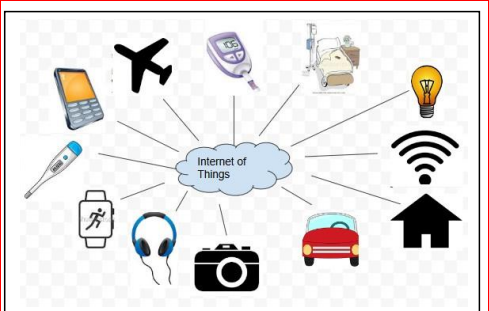
\includegraphics[width=10cm]{iot_sensors.png}
	\caption{سنسورهای اینترنت اشیاء}
\end{figure}


\subsection{اهمیت و کاربرد}
اینترنت اشیاء با دارابودن قابلیت بسیار بالا برای بهره‌ور نمودن کسب و کارها در حوزه‌های مختلف از جمله صنایع به عنوان انقلاب آتی در فناوری اطلاعات و ارتباطات معرفی شده‌است. این بهره‌وری در زمنیه بروز نوآوری و ارائه قابلیت‌های نو برای کسب‌و کارها است. صنایع مختلف در خصوص اینترنت اشیاء واکنش‌های مختلفی را نشان داده‌اند اما آنچه واضح است این است که اینترنت اشیاء در تمامی کسب‌و کارها و صنایع دارای کاربرد است. این کاربردها در برخی صنایع مانند بهداشت و حوزه سلامت و یا حمل و نقل پیشرفت چشمگیری داشته اما در صنایع دیگر همچون کشاورزی و دامداری در حال توسعه است در واقع تولید داده‌ها بر مبنای اینترنت اشیاء از ارکان اصلی در حوزه مه‌داده‌ها و علم داده‌ها خواهد بود. لذا استفاده از مفاهیم و مدل‌های آماری که در علم داده‌ها مورد استفاده قرار می‌گیرند به خوبی می‌توانند در این‌گونه داده‌ها مورد استفاده قرار گیرند.
\subsection{چالش ها}
چالش های مختلفی در زمینه اکوسیستم اینترنت اشیاء وجود دارد اما به صورت عمده می‌توان این موارد را به ۲ لایه فیزیکی و نرم افزاری تقسیم‌بندی کرد. به دلیل وجود داشتن انواع متنوع و مختلف از سنسورها در این زمینه باعث تولید بی وقفه داده و ایجاد داده‌های مختلف با ساختار‌های متفاوت می‌شود که تمرکز این پایان‌نامه به بررسی روش‌های مختلف تحلیل این‌ داده‌ها و انجام تحلیل بر روی یک نوع داده اینترنت اشیاء می‌باشد.
 
\section{ساختار داده‌ها}
کلان داده‌ها می‌توانند به اشکال مختلف، از جمله داده‌های ساختاریافته و غیرساخت‌یافته مانند داده‌های مالی، فایل‌های متنی، فایل‌های چندرسانه‌ای باشند. برخلاف بسیاری از تحلیل‌های سنتی داده‌ها که توسط سازمان‌ها انجام می‌شود، بیشتر داده‌های بزرگ ماهیتی بدون ساختار یا نیمه ساختار یافته دارند که برای پردازش و تجزیه و تحلیل به تکنیک‌ها و ابزارهای مختلفی نیاز دارد. محیط‌های محاسباتی توزیع‌شده و معماری‌های پردازش انبوه موازی (MPP) که دریافت و تجزیه و تحلیل داده‌های موازی را امکان‌پذیر می‌کنند، رویکرد ترجیحی برای پردازش چنین داده‌های پیچیده هستند.

شکل 
\ref{g_data_structured}
چهار نوع ساختار داده را نشان می‌دهد که ۸۰ تا ۹۰ درصد رشد داده‌های آینده از انواع داده‌های غیر ساختاریافته است. اگرچه این چهار نوع ساختار با هم متفاوت هستند اما معمولا با یکدیگر مخلوط می‌شوند.به عنوان مثال یک سیستم مدیریت پایگاه داده رابطه‌ای کلاسیک(RDBMS) ممکن است گزارش‌های تماس را برای یک مرکز تماس پشتیبانی نرم‌افزار ذخیره کند.RDBMS ممکن است ویژگی های تماس‌های پشتیبانی را به عنوان داده‌های ساختار یافته ذخیره کند اما ممکن است علاوه‌بر این موضوع سیستم دارای داده‌های بدون ساختار،شبه یا نیمه ساختاریافته باشد مانند تاریخچه چت مشتری، فایل صوتی مکالمات تلفنی، تصویر رسید مشتری و غیره باشد.

\begin{figure}[htbp]
\centering
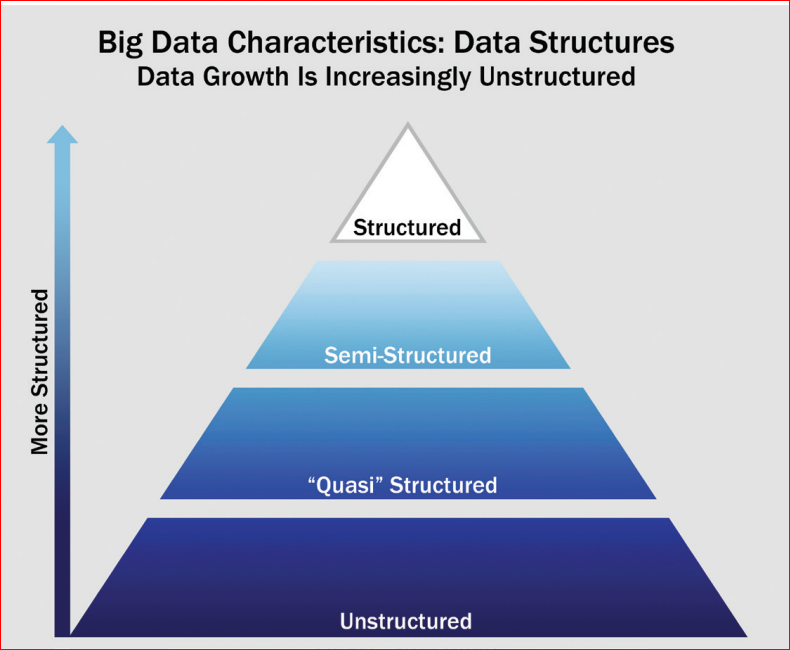
\includegraphics[width=10cm]{data_structured.png}
\caption{رشد داده‌ها}
\label{g_data_structured}
\end{figure}

روش‌های شناخته‌شده و مرسوم و متداولی برای تجزیه و تحلیل داده‌های ساختار یافته وجود دارد اما تکنیک‌های متفاوتی برای مقابله چالش‌های تجزیه و تحلیل داده‌های نیمه ساختار‌یافته، شبه ساختار‌یافته، و داده‌های بدون ساختار مورد نیاز است.
در ادامه به معرفی و بررسی هرکدام از این نوع داده‌ها می‌پردازیم.
\cite{emc2015data}

\subsection{داده ساختار‌یافته}

داده‌های ساختار‌یافته
\LTRfootnote{Structured data}
داده‌هایی هستند که فرمت مناسبی دارند و به راحتی می‌توان اطلاعات از آن‌ها استخراج کرد. داده‌های ساختاریافته را می‌توان در ستون‌ها و ردیف‌ها ذخیره کرد. این داده‌ها به راحتی توسط ابزارهای داده‌کاوی مورد استفاده قرار می‌گیرد و می‌تواند در سیستم مدیریت پایگاه داده رابطه‌ای (RDBMS) ذخیره شود. عمدتا پایگاه داده رابطه‌ای سنتی برای ذخیره داده‌های ساختاریافته استفاده می‌شود. داده‌های تراکنش، فایل‌های CSV، فایل‌های اکسل از انواع داده‌های ساختار یافته می‌باشند.

\cite{verma2020}


\begin{figure}[htbp]
	\centering
	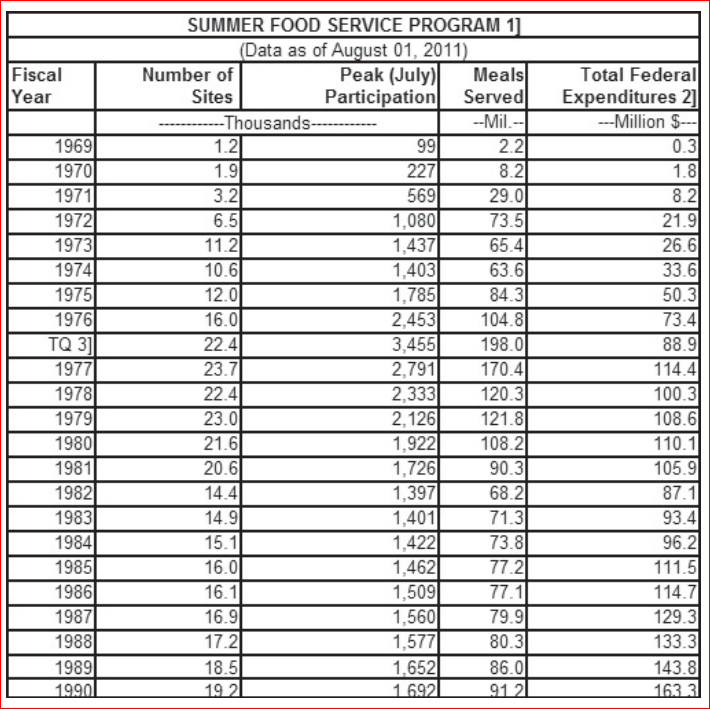
\includegraphics[width=10cm]{exp_structured_data.png}
	\caption{مثال داده ساختاریافته}
\end{figure}

\subsection{داده نیمه‌ساختار یافته}
داده نیمه ساختار یافته
\LTRfootnote{Semi-structured data}
از ساختار رسمی ندمل داده‌های مربوط به پایگاه داده رابطه‌ای که شامل سطر و ستون هستند پیروی نمی‌کنند. پیشرفت در استفاده از اینترنت حضور داده‌های نیمه‌ساختاری راا افزایش می‌دهد.فایل‌های داده متنی با الگوی قابل تشخیص که تجزیه را امکان‌پذیر میکند مانند فایل‌های داده زبان نشانه‌گذاری توسعه‌یافته
\LTRfootnote{XML}
یا فایل‌های نمادگذاری اشیاء در جاوا‌اسکریپت
\LTRfootnote{JSON}
از این نوع داده‌ها می‌باشند.
\begin{figure}[htbp]
	\centering
	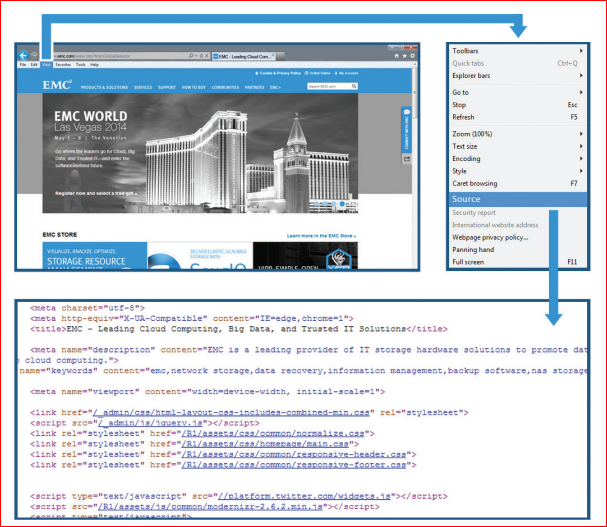
\includegraphics[width=10cm]{exp_semistructured.png}
	\caption{مثال داده نیمه ساختاریافته}
\end{figure}

\subsection{داده شبه ساختاریافته}
داده‌های شبه ساختاریافته
\LTRfootnote{Quasi-structured data}
داده‌های متنی با قالب‌های داده نامنظم که می‌توانند با تلاش، ابزار و زمان قالب‌بندی شوند به عنوان مثال، داده‌های جریان کلیک وب که ممکن است حاوی ناسازگاری در مقادیر و قالب‌های داده باشد از این نوع داده‌ها می‌باشد. شکل
\ref{r_exp_quasi}
را ببینید.
\begin{figure}[H]
	\centering
		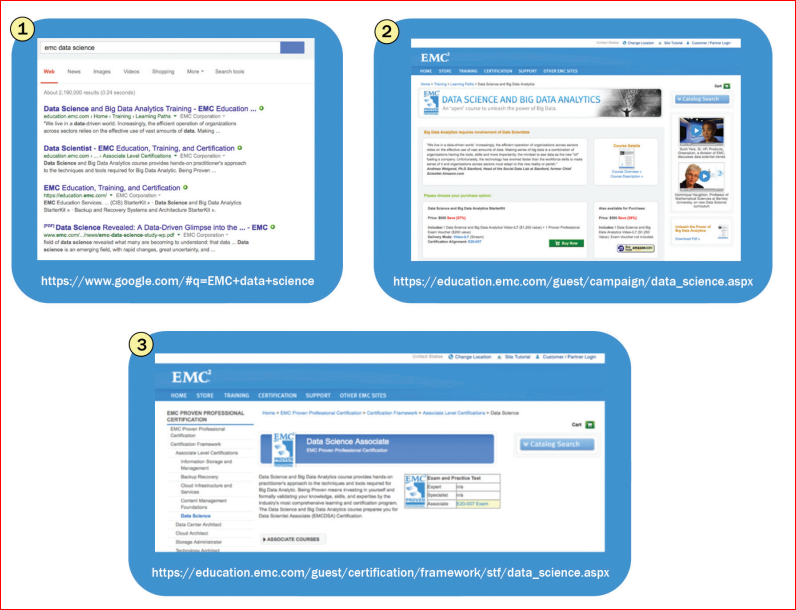
\includegraphics[width=8cm]{exp_quasi_structured.png}
	\caption{مثال داده شبه ساختاریافته}
\label{r_exp_quasi}
\end{figure}

\subsection{داده بدون ساختار}
داده‌ بدون ساختار
\LTRfootnote{Unstructured data}
داده‌هایی هستند که مدل مناسبی ندارند و یا به روش مناسب سازماندهی نشده‌اند.درک و تجزیه و تحلیل این داده‌ها به دلیل اینکه در قالب جدولی نیستند سخت است.انواع این داده‌ها عبارتند از: اسناد متنی، اسناد قابل حمل
\LTRfootnote{PDF}
تصاویر، صوت و فایل‌های ویدئو باشند.

\begin{figure}[h]
	\centering
	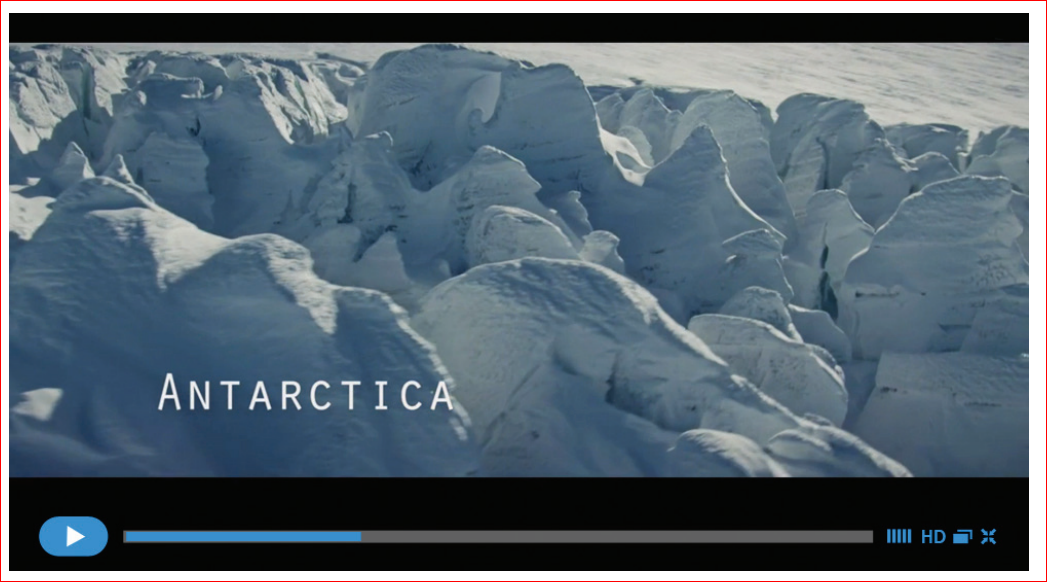
\includegraphics[width=10cm]{exp_unstructured_data.png}
	\caption{ویدئویی در مورد سفر قطب جنوب نمونه‌ای از داده بدون ساختار}
\end{figure}

\section{فرآیند تحلیل داده اینترنت اشیاء}
مقدار داده تولید شده توسط سنسورهای اینترنت اشیاء بسیار زیاد است و به طور مداوم تولید می‌شود. داده‌های تولید شده به صورت بدون ساختار هستند و این داده‌ها باید به شکل ساختاری برای استخراج دانش از آن تبدیل شوند.سیستم پیشنهادی با استفاده از الگوریتم های یادگیری ماشین و یادگیری عمیق، داده‌های بدون ساختار را به داده‌های ساختاریافته تبدیل می‌کند. شکل
\ref{flochart}
نمودار فرآیند سیستم پیشنهادی جهت تحلیل داده بدون ساختار است.
ابتدا داده‌ها را از منابع مد نظر وارد می‌کنیم،‌ سپس باید پاکسازی داده‌ها برای هر مجموعه‌ داده انجام شود. پاکسازی داده‌ها شامل استاندارد سازی داده‌ها، بررسی موارد گمشده و داده‌های دورافتاده و مرتب کردن داده‌ها می‌باشد. سپس داده‌ها را به داده‌های آموزشی و آزمایشی تقسیم می‌کنیم. داده‌های آموزشی باید با دقت طبقه‌بندی شوند، مدل نباید بیش برازش یا کم برازش شود. با اعمال الگوریتم های مختلف دقت مدل را با پارامترهای مختلف بررسی کنید تا دقت بالایی به‌دست آید. و در انتها تجسم داده‌ها برای استخراج دانش از داده‌های خام مانند نمودار میله‌ای، نمودار پراکندگی و غیره انجام می‌شود.

\begin{figure}[H]
	\centering
	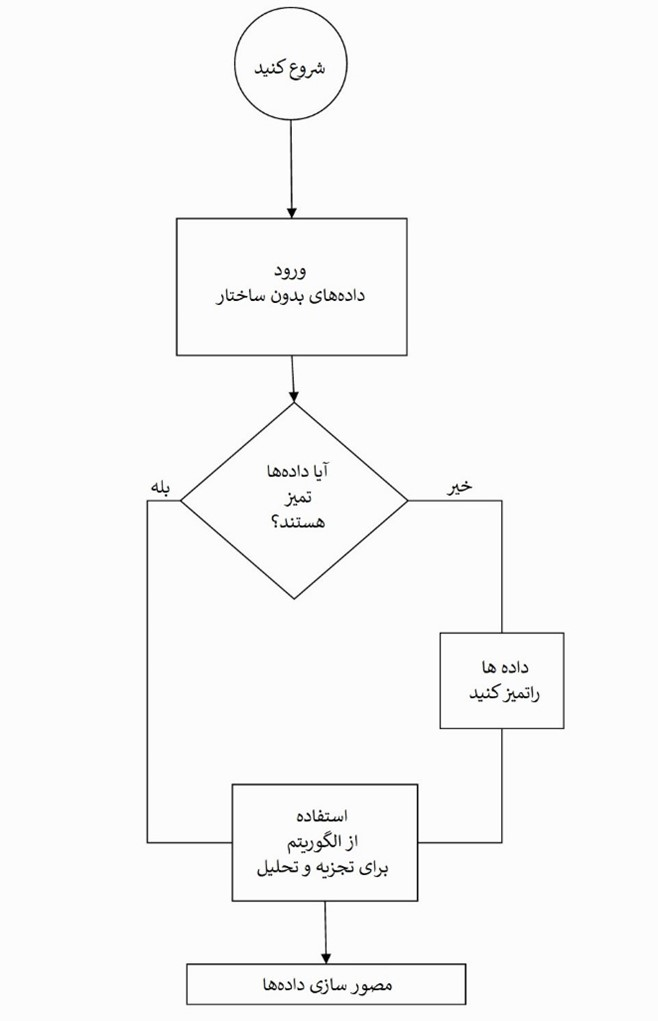
\includegraphics[width=10cm]{flochart.jpg}
	\caption{نمودار روند تحلیل داده‌ بدون ساختار}
	\label{flochart}
\end{figure}

\section{هوش مصنوعی}
هوش مصنوعی تکنیکی است که رایانه‌ها یا ماشین‌ها را قادر می‌سازد تا توانایی انسان برای انجام، رفتار یا عملکرد را تقلید کنند. هوش مصنوعی می تواند از داده‌های گذشته بیاموزد و قادر به تشخیص الگوها و رفتار است. این امکان را برای ماشین فراهم می کند که از تجربه درس بگیرد و رفتار خود را تحمل کند. اصطلاح هوش مصنوعی در سال 1956 توسط جان مک کارتی
\LTRfootnote{McCarthy}
 ابداع شد. زمینه های بین رشته‌ای زیادی تحت هوش مصنوعی وجود دارد. در شکل
 \ref{exp_ai_ml}
 موقعیت یادگیری ماشین
 \LTRfootnote{Machine Learning}
  و یادگیری عمیق
   \LTRfootnote{Deep Learning}
   را در ارتباط با هوش مصنوعی نشان می‌دهد.
 
 \begin{figure}[H]
 	\centering
 	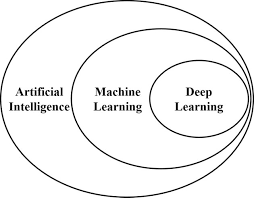
\includegraphics[width=5cm]{Example of AI and ML.png}
 	\caption{ارتباط یادگیری ماشین و یادگیری عمیق}
 	\label{exp_ai_ml}
 \end{figure}
اصطلاح هوش مصنوعی بسیار گسترده است در حالی که یادگیری ماشین شاخه‌ای از هوش مصنوعی است. یادگیری ماشین اولین بار در سال 1959 توسط آرتور ساموئل ابداع شد که از روش های آماری استفاده می کند تا ماشین ها را قادر سازد عملکرد و رفتار خود را از طریق تجربه بهبود بخشند. با توجه به شکل \ref{exp_ai_ml}، یادگیری عمیق زیر شاخه ای از یادگیری ماشین است. این اصطلاح در سال 1986 توسط رینا دچتر به جامعه یادگیری ماشین و در سال 2000 توسط ایگور آیزنبرگ به شبکه عصبی مصنوعی معرفی شد.
\cite{alaskar2021machine}
در ادامه به مرور کلی بر مفاهیم اساسی یادگیری عمیق و یادگیری ماشین می‌پردازیم.
%